\section{Experimental results}
\label{sec:results}

\subsection{Main experiments}

Fifteen runs were executed; the six that changed the course of the project are in
Table~\ref{tab:experiments}.

\begin{table}[ht]
    \centering
    \caption{The main experiments. Dice and PQ at each run's own operating point,
    official metric at native $2048^2$; the first three predate that protocol and
    are reported at threshold $0.5$ (marked *).}
    \label{tab:experiments}
    \small\begin{tabular}{clrrl}
        \toprule
        Exp. & One variable & Dice & PQ & Outcome \\
        \midrule
        1 & U-Net from scratch, $512^2$           & 0.6415* & --      & baseline \\
        2 & ImageNet ResNet18 encoder             & 0.6552* & 0.2505* & calibration, +1 pt Dice \\
        3 & topology loss (Tversky + clDice)      & 0.4937* & 0.0618* & \textbf{falsified}, instructive \\
        5 & resolution $512 \to 1024$             & 0.6665  & 0.4022  & largest single gain \\
        8 & $\to 1536$, D4 TTA, confidence gate   & 0.6729  & \textbf{0.4264} & best PQ (single model) \\
        13 & native 2048, random 1536 windows     & \textbf{0.6815} & 0.3930  & best Dice -- \textbf{delivered} \\
        \bottomrule
    \end{tabular}
\end{table}

\textbf{Baseline and transfer (1--2).} The from-scratch U-Net reaches Dice 0.6415
at the last epoch, still underfitted, with its best threshold at the edge of the
search grid -- badly calibrated probabilities that point at the encoder. The
pre-trained encoder adds a point of Dice and, more usefully, flattens the
threshold--Dice curve: for an inference configuration that must be frozen before
seeing the test set, calibration is worth more than the point.

\textbf{The instructive failure (3).} Replacing half the loss with recall-biased
Tversky~\cite{tversky} plus clDice~\cite{cldice} collapses validation to Dice 0.49
and PQ 0.06 while the training loss decreases: the model optimises the wrong thing
successfully. The post-mortem matters more than the number -- at $512^2$ many
filaments are one or two pixels wide, so the soft skeleton clDice needs is noise on
exactly the structures it was meant to protect. A \emph{scale} problem disguised as
a loss problem, and the reason experiment 5 exists.

\textbf{Resolution (5, 8).} Nothing changes but the input size, $512 \to 1024$:
Dice gains one point while PQ jumps $+28\%$ relative. The asymmetry is the finding
-- resolution barely changes how much of the disk is covered correctly, and changes
a great deal about how many filaments exist as recognisable objects. Pushing to
$1536$ with test-time averaging over the eight square symmetries and a confidence
gate gives the best instance score of the study.

\textbf{Native pixels (13).} Training on random $1536^2$ windows of the untouched
$2048^2$ frame removes the last resize from the pipeline. It \emph{loses} on
recognition -- windows give up full-disk context -- and \emph{wins} on mask
quality: Dice \textbf{0.6815}, the highest of the study, with training at 3.04~GB
and inference at 2.50~GB, the only configuration inside the assignment's memory
bonus on both counts (Figure~\ref{fig:curves}).

\textbf{Measured and rejected.} Nine further single-variable runs and a dozen
post-hoc mechanisms were falsified, each with its number: scale jitter ($-0.019$
PQ), a detect-then-refine cascade ($-0.025$), soft consensus targets ($-0.033$),
clDice retested at $1536$ where its premise was finally valid ($-0.013$), an
instance-balanced Dice as dominant loss term (false-positive control collapsed), a
positive-class weight in the BCE (it cured the measured under-segmentation and paid
for it in hallucinations), per-component thresholds and dilation, and three
flavours of post-hoc filament merging whose aggregate gains died under
cross-selection.

\begin{figure}[ht]
    \centering
    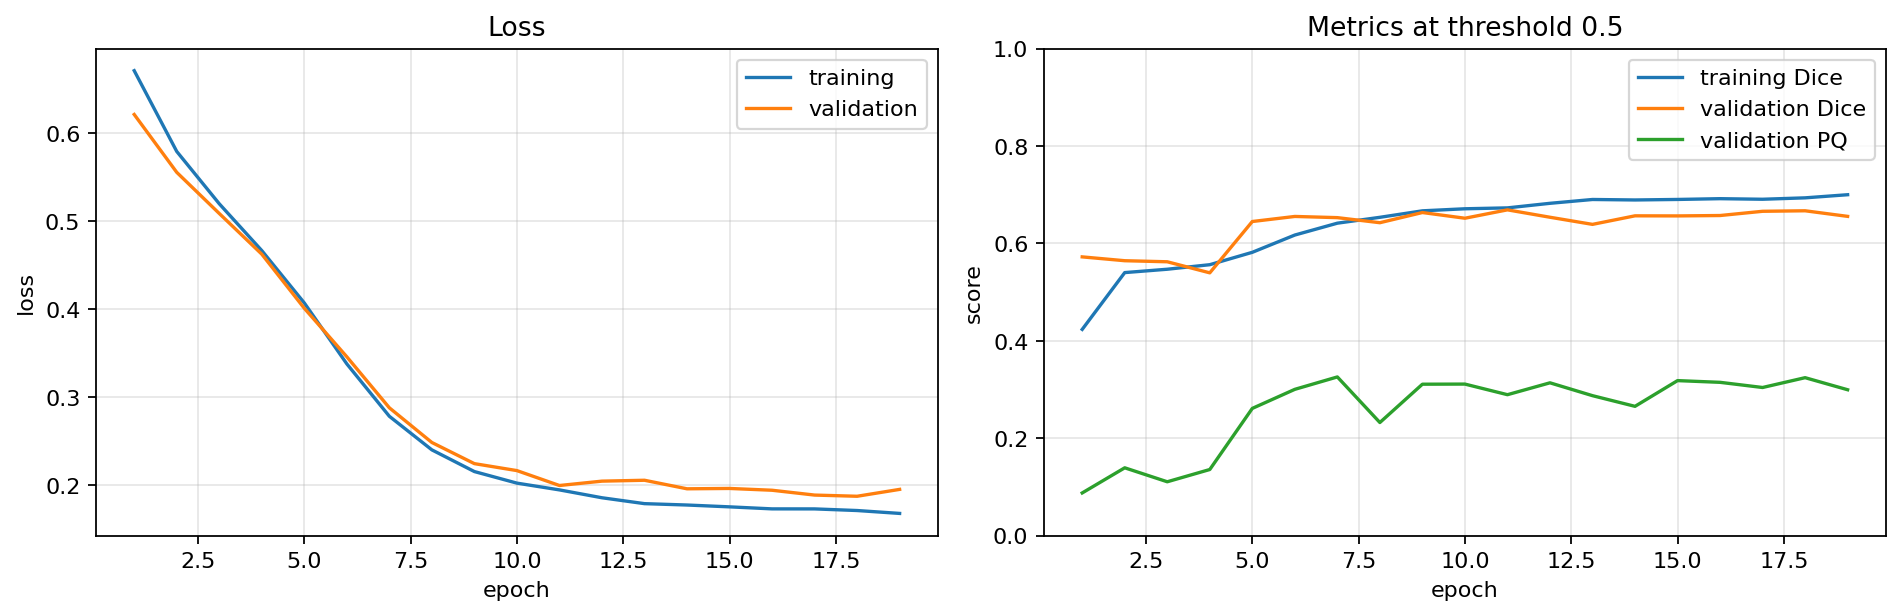
\includegraphics[width=0.72\linewidth]{../experiments/13/plots/training_curves.png}
    \caption{The delivered model (experiment 13) in training: loss and metrics at
    threshold 0.5. The operating point is selected afterwards.}
    \label{fig:curves}
\end{figure}

\subsection{Post-processing and operating point}
\label{sec:operating}

The network outputs one probability per pixel. Turning that map into the final
filament instances takes four \emph{post-processing hyperparameters} -- together
they form the \emph{operating point}, selected with a joint grid search on the
validation set (never on the test set) because they interact:

\begin{itemize}\itemsep0pt
    \item \textbf{threshold} ($0.50$ in the delivered configuration): a pixel with
          probability above it becomes filament, below it background;
    \item \textbf{morphological closing} ($1$ iteration): fills one-pixel gaps, so
          a filament the network split in two becomes one component again -- two
          false positives and one false negative turn into a single true positive;
    \item \textbf{minimum component size} ($384$ pixels at $2048^2$): a connected
          component smaller than this is discarded entirely, because every small
          spurious blob costs a full false positive in PQ while adding almost
          nothing to Dice;
    \item \textbf{confidence gate} ($0.90$): a component survives only if at least
          one of its pixels exceeds this probability. The threshold alone performs
          two roles at once -- deciding \emph{which} components exist and their
          \emph{extent} -- so raising it to remove weak blobs also thins every real
          filament; the gate takes over the existence decision and leaves the
          shapes exactly as the threshold drew them.
\end{itemize}

\begin{wrapfigure}{r}{0.42\textwidth}
    \vspace{-1.2em}
    \centering
    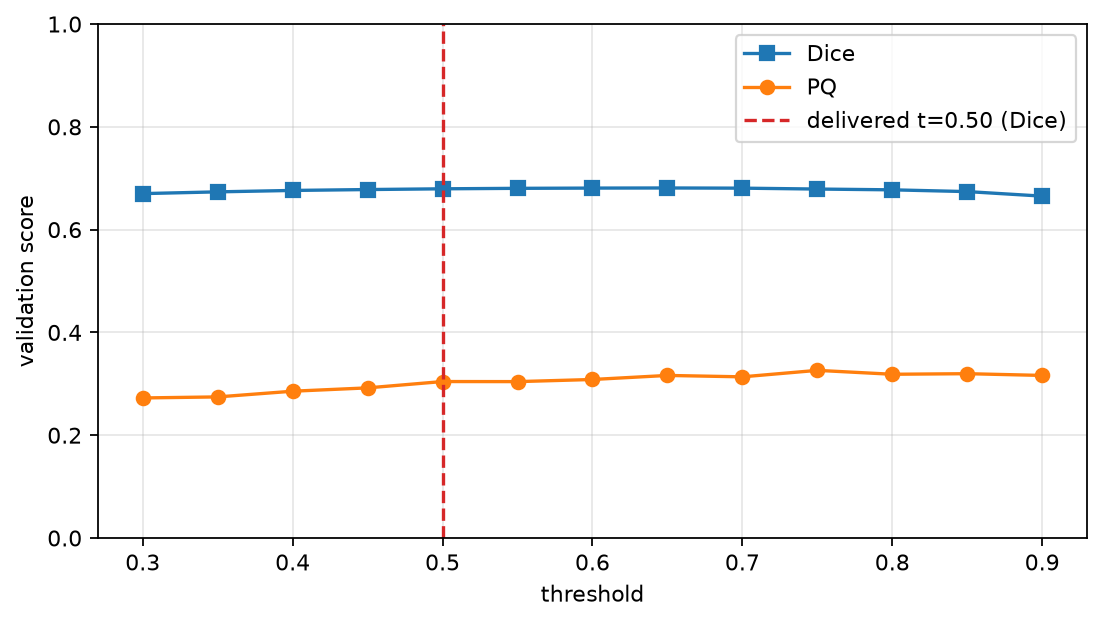
\includegraphics[width=0.40\textwidth]{../experiments/13/plots/threshold_search.png}
    \caption{Validation Dice and PQ against the threshold for the delivered model,
    without post-processing: the two metrics peak at different points.}
    \label{fig:threshold}
    \vspace{-1em}
\end{wrapfigure}

Everything is scored at the native $2048^2$, because that is where the submission
is written: a minimum size tuned at training resolution means something else at
native scale, and the number of connected components is not preserved by resizing a
mask. Measured when this protocol was introduced, selecting at native resolution
against the official definition was worth $+0.020$ Dice and $+0.006$ PQ over the
configuration that would otherwise have shipped -- free, with no retraining.

The same search grid yields one point per objective. The \textbf{delivered
configuration} is frozen on Dice, the assignment's score: threshold $0.50$, closing
$1$, minimum size $384$, gate $0.90$, giving \textbf{Dice 0.6815} (PQ 0.393) on
validation. Cross-selection puts the cost of the finer grid at $0.0024$, with both
halves of the validation set selecting the same threshold and gate. The PQ-optimal
point of the same model (0.407) and of the study (0.4264, experiment 8) are
recorded alongside in the experiment artifacts.
